\documentclass{article}
\usepackage{circuitikz}
% http://mirrors.ibiblio.org/CTAN/graphics/pgf/contrib/circuitikz/doc/circuitikzmanual.pdf
\begin{document}
	\begin{center}
\begin{circuitikz}[]
	 \draw (0,0) node[flipflop JK]{JK};
	 \ctikzset{multipoles/flipflop/clock wedge size=0.1}
	 \draw (2.3,0) node[flipflop JK]{JK};
	 \ctikzset{multipoles/flipflop/clock wedge size=0.4}
	 \draw (4.6,0) node[flipflop JK]{JK};
	 \end{circuitikz}
	 
	 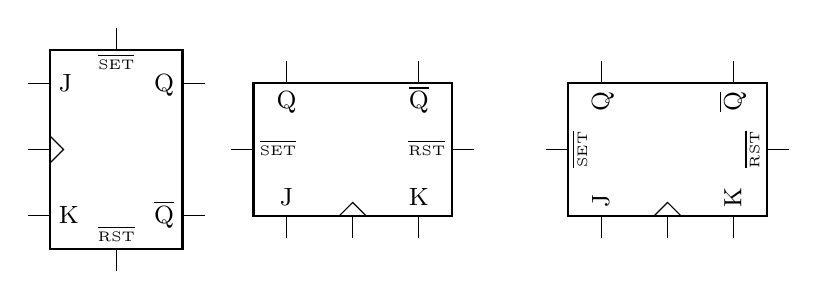
\begin{tikzpicture}
	 	 \draw (0,0) node[flipflop JK, add async SR]{};
	 	 \draw (3,0) node[flipflop JK, add async SR, rotate=90]{};
	 	 \draw (7,0) node[flipflop JK, add async SR, rotate=90, rotated numbers]{};
	  \end{tikzpicture}
	 	
\begin{circuitikz}[]
 \ctikzset{logic ports=european,
	 tripoles/european not symbol=ieee circle}
	 \draw (0,0) node[nand port](A){} (A.out) to[short] ++(0.5,0)
	 
	 node[flipflop JK, dot on notQ, anchor=pin 2]{JK};
	 
	 \ctikzset{logic ports=european, tripoles/european not symbol=circle}
	 
	 \draw (0,-3) node[nand port](A){}	 (A.out) to[short] ++(0.5,0)
	 node[flipflop JK, dot on notQ, anchor=pin 2]{JK};
	 \end{circuitikz}		 	
	 	
	\end{center}
\end{document}